\chapter{Kerr black hole}
\label{s:ker}
\index{Kerr!black hole}

\minitoc

\section{Introduction}

\section{The Kerr solution}

\subsection{Expression in Boyer-Lindquist coordinates}

The Kerr solution depends on two constant real non-negative parameters:
\begin{itemize}
\item the \defin{mass parameter}\index{mass!parameter of Kerr solution} $m > 0$, to be
interpreted in Sec.~?? as the spacetime total mass;
\item the \defin{spin parameter}\index{spin!parameter of Kerr solution} $a \geq 0 $,
to be interpreted in Sec.~?? as the reduced angular momentum  $a=J/m$, $J$ being the
spacetime total angular momentum.
\end{itemize}
In this part, we focus on Kerr solutions for which
\be \label{e:ker:a_lower_m}
    0 < a < m .
\ee
The Kerr solution is usually presented in the so-called
\defin{Boyer-Lindquist coordinates}\index{Boyer-Lindquist coordinates}
$(t,r,\th,\ph)$. Except for the standard singularities of the
spherical coordinates $(\th,\ph)$ on $\SS^2$ at $\theta\in\{0,\pi\}$,
we may consider that the Boyer-Lindquist coordinates cover the manifold
$\R^2\times\SS^2$, with $t$ spanning $\R$, $r$
spanning\footnote{NB: $r$ does not only span $(0,+\infty)$ as in the case of
the standard spherical coordinates $(r,\th,\ph)$ on $\R^3$.} $\R$ and
$\th$ spanning $(0,\pi)$ and $\ph$ spanning $(0,2\pi)$. Hence
$(t,r)$ is a Cartesian chart covering $\R^2$ and $(\th,\ph)$ is the standard
spherical chart of $\SS^2$.

The spacetime manifold can then be taken as an open subset $\M_{\rm BL}$
of $\mathbb{R}^2\times\mathbb{S}^2$ formed by the disjoint union of three components:
\begin{subequations}
\begin{align}
    \M_{\rm BL} & :=  \M_{\rm I} \cup \M_{\rm II} \cup \M_{\rm III} , \\
    \M_{\rm I} & :=  \R\times(r_+,+\infty)\times\SS^2 \label{e:ker:def_M_I}\\
    \M_{\rm II} & :=  \R\times(r_-,r_+)\times\SS^2 \\
    \M_{\rm III} & :=  \R\times(-\infty,r_-)\times\SS^2 \setminus \ring, \label{e:ker:def_M_III}
\end{align}
\end{subequations}
where
\be \label{e:ker:def_r_pm}
    \encadre{r_+ := m + \sqrt{m^2-a^2}} \quad\mbox{and}\quad  \encadre{r_- := m - \sqrt{m^2-a^2}}
\ee
and $\ring$ is the subset of $\R^2\times\SS^2$ defined in terms of the Boyer-Lindquist coordinates $(t,r,\th,\ph)$ by
\be \label{e:ker:def_ring}
    \ring = \left\{ p \in \R^2\times\SS^2,
        \quad r(p) = 0 \ \mbox{and}\ \th(p) = \frac{\pi}{2} \right\} .
\ee
Note that thanks to the constraint (\ref{e:ker:a_lower_m}), $r_+$ and $r_-$
are well defined and obey
\be
    0 < r_- < m < r_+ < 2 m .
\ee
Note also that $\ring$ is spanned by the coordinates $(t,\ph)$ and is diffeomorphic to the 2-dimensional cylinder $\R\times\SS^1$:
\be
    \ring \simeq \R\times\SS^1 .
\ee
This is so because $r=0$ is \emph{not} a peculiar value of $r$ in $\R^2\times\SS^2$.
In view of Eqs.~(\ref{e:ker:def_M_I})-(\ref{e:ker:def_M_III}) and (\ref{e:ker:def_ring}), it is clear that
the various connected components of $\M_{\rm BL}$ are defined in terms of the
Boyer-Lindquist coordinates $(t,r,\th,\ph)$ by
\begin{subequations}
\begin{align}
  \forall p \in  \M_{\rm BL},\quad p \in \M_{\rm I} & \iff r(p) > r_+ \\
    \quad p \in \M_{\rm II} & \iff r_- < r(p) < r_+ \\
    \quad p \in \M_{\rm III} & \iff r(p) < r_-\ \mbox{and}\
    \left( r(p) \not=0 \ \mbox{or}\ \theta(p) \not=\frac{\pi}{2} \right) .
\end{align}
\end{subequations}


The \defin{Kerr metric}\index{Kerr!metric} is defined by the following
components in terms of the Boyer-Lindquist coordinates $(t,r,\th,\ph)$:
\be \label{e:ker:metric_BL}
    \encadre{
    \begin{array}{ll}
    g_{\mu\nu}\,  \D x^\mu \D x^\nu  = &
    \displaystyle - \left( 1 - \frac{2m r}{\rho^2} \right) \, \D t^2
    - \frac{4 a m  r \sin^2\th}{\rho^2} \,  \D t\, \D\ph
    + \frac{\rho^2}{\Delta} \, \D r^2  \\[2ex]
    & \displaystyle + \rho^2 \D \th^2
    + \left( r^2 + a^2 + \frac{2 a^2 m r \sin^2\th}{\rho^2} \right)
    \sin^2\th \, \D \ph^2 ,
    \end{array}
    }
\ee
with
\be \label{e:ker:def_rho2}
    \encadre{\rho^2 := r^2 + a^2 \cos^2\th}
\ee
and
\be \label{e:ker:def_Delta}
    \encadre{\Delta := r^2 - 2 m r + a^2 = (r-r_-)(r-r_+)} .
\ee
By means of a computer algebra system (cf. Appendix~\ref{s:sam}),
it is easy to check that $\left(\M_{\rm BL},\w{g}\right)$ with $\w{g}$ given
by (\ref{e:ker:metric_BL}), is a solution of Einstein equation (\ref{e:bas:Einstein_eq})
in vacuum ($\w{T}=0$) and with a vanishing cosmological constant ($\Lambda=0$).

\subsection{Basic properties}

Various properties of the Kerr metric are immediate:
\begin{itemize}
\item For $r\rightarrow+\infty$ or $r\rightarrow-\infty$, one has $\rho^2\sim r^2$ and
$\rho^2/\Delta \sim (1-2m/r)^{-1}$,
and $4 a m  r / \rho^2\,  \D t\, \D\ph \simeq 4 a m/r^2 \,  \D t\, r\D\ph$,
so that the metric (\ref{e:ker:metric_BL}) becomes
\be \label{e:ker:asympt_metric}
    g_{\mu\nu}\,  \D x^\mu \D x^\nu  \simeq  - \left( 1 - \frac{2m}{r} \right) \, \D t^2
    + \left( 1 - \frac{2m}{r} \right) ^{-1} \D r^2
    + r^2 \left( \D \th^2 + \sin^2\th  \, \D \ph^2 \right)
    + O\left(\frac{1}{r^2}\right)
\ee
For $r>0$, we recognize the Schwarzschild metric\index{Schwarzschild!metric} expressed
in Schwarzschild-Droste coordinates [cf. Eq.~??].
For $r<0$, the change of coordinate $r'=-r$ leads also to the Schwarzschild metric
but with a negative mass parameter $m'=-m$.
Hence, the Kerr metric has (at least) two asymptotically flat ends: one in
$\M_{\rm I}$ for $r\rightarrow + \infty$ and one in $\M_{\rm III}$ for
$r\rightarrow - \infty$.
\item Since in (\ref{e:ker:metric_BL}), all the metric components $g_{\alpha\beta}$ are independent from $t$ and $\ph$, the
spacetime $(\M_{\rm BL},\w{g})$ admits two isometries, generated by the Killing
vectors
\be
    \encadre{\w{\xi} := \wpar_t} \quad\mbox{and}\quad
    \encadre{\w{\eta} := \wpar_\ph}.
\ee
Since $t$ spans $\R$, the isometry group generated by $\w{\xi}$ is clearly
the translation group\index{translation!group}\index{group!translation --} $(\R,+)$. Moreover, in
view of (\ref{e:ker:asympt_metric}), we have $\w{\xi}\cdot\w{\xi} = g_{tt} < 0$
as $r\rightarrow +\infty$, which means that the Killing vector $\w{\xi}$
is asymptotically timelike. Given the definition of stationarity stated in
Sec.~\ref{s:glo:def_station}, we conclude that the Kerr spacetime is
stationary.
On the other side, given the definition of $\ph$ as an azimuthal coordinate
on $\SS^2$, the isometry group generated by $\w{\eta}$ is the rotation
group\index{rotation!group}\index{group!rotation --} $\mathrm{SO}(2) = \mathrm{U}(1)$.
Hence, the Kerr spacetime is axisymmetric.
\item When $a\not=0$, as we have assumed in (\ref{e:ker:a_lower_m}), the
Kerr spacetime is not static, since the stationary Killing vector $\w{\xi}$
is not orthogonal to the hypersurfaces $t=\mathrm{const}$. Indeed
the vector $\w{\eta}$ is tangent to these hypersurfaces and from
(\ref{e:ker:metric_BL}),
\[
    a\not=0 \ \Longrightarrow \ \w{\xi}\cdot\w{\eta} = g_{t\ph} \not=0 .
\]
\item When $a\rightarrow 0$, we have $r_+\rightarrow 2m$, $r_-\rightarrow 0$,
$\rho^2\sim r^2$, and $\rho^2/\Delta \sim (1-2m/r)^{-1}$, and we see on
(\ref{e:ker:metric_BL}) that the Kerr metric reduces to the Schwarzschild metric.
\end{itemize}

\subsection{Ergoregions}

Let us investigate the causal character of the stationary Killing vector $\w{\xi}$.
We have, according to (\ref{e:ker:metric_BL}) and (\ref{e:ker:def_rho2}),
\[
    \w{\xi}\cdot\w{\xi} = g_{tt} = - 1 + \frac{2m r}{r^2 + a^2\cos^2\th} .
\]
Thus
\[
    \w{\xi}\ \mbox{timelike} \iff r^2 - 2 m r + a^2\cos^2\th > 0
        \iff r < r_{\E^-}(\theta) \quad\mbox{or}\quad  r > r_{\E^+}(\theta) ,
\]
with
\be
    r_{\E^\pm}(\theta) := m \pm \sqrt{m^2 - a^2\cos^2\th} .
\ee
Comparing with (\ref{e:ker:def_r_pm}), we note that
\be
    0 \leq r_{\E^-}(\theta) \leq r_- \leq m \leq r_+ \leq r_{\E^+}(\theta)
        \leq 2 m ,
\ee
with
\begin{subequations}
\begin{align}
 & r_{\E^-}(\pi/2) = 0 \\
 & r_{\E^-}(0)  = r_{\E^-}(\pi) = r_- \\
 & r_{\E^+}(0)  = r_{\E^+}(\pi) = r_+ \\
 & r_{\E^+}(\pi/2) = 2 m .
\end{align}
\end{subequations}
Given the definition of $\M_{\rm I}$, $\M_{\rm II}$ and $\M_{\rm III}$, we conclude that
\begin{itemize}
\item $\w{\xi}$ is timelike in the region of $\M_{\rm I}$ defined by $r>r_{\E^+}(\theta)$
and in the region of $\M_{\rm III}$ defined by $r<r_{\E^-}(\theta)$;
\item $\w{\xi}$ is null on the hypersurface $\E^+$ of $\M_{\rm I}$ defined by
$r=r_{\E^+}(\theta)$
and on the hypersurface $\E^-$ of $\M_{\rm III}$ defined by $r=r_{\E^-}(\theta)$;
\item $\w{\xi}$ is spacelike in all $\M_{\rm II}$ and in the region
$\mathscr{G}^+$ of $\M_{\rm I}$
defined by $r<r_{\E^+}(\theta)$, as well as
in the region $\mathscr{G}^-$ of $\M_{\rm III}$ defined by $r>r_{\E^-}(\theta)$.
\end{itemize}
According to the nomenclature introduced in Sec.~\ref{s:glo:strong_rigidity},
one calls $\E^+$ (resp. $\E^-$) the
\defin{outer ergosphere}\index{outer!ergosphere}\index{ergosphere!outer --}
(resp. \defin{inner ergosphere}\index{inner!ergosphere}\index{ergosphere!inner --})
and $\mathscr{G}^+$ (resp. $\mathscr{G}^-$) the
\defin{outer ergoregion}\index{outer!ergoregion}\index{ergoregion!outer --}
(resp. \defin{inner ergoregion}\index{inner!ergoregion}\index{ergoregion!inner --}).
\begin{remark}
Sometimes the word \defin{ergosurface}\index{ergosurface} is used instead of
\emph{ergosphere}.
\end{remark}

\begin{figure}
\centerline{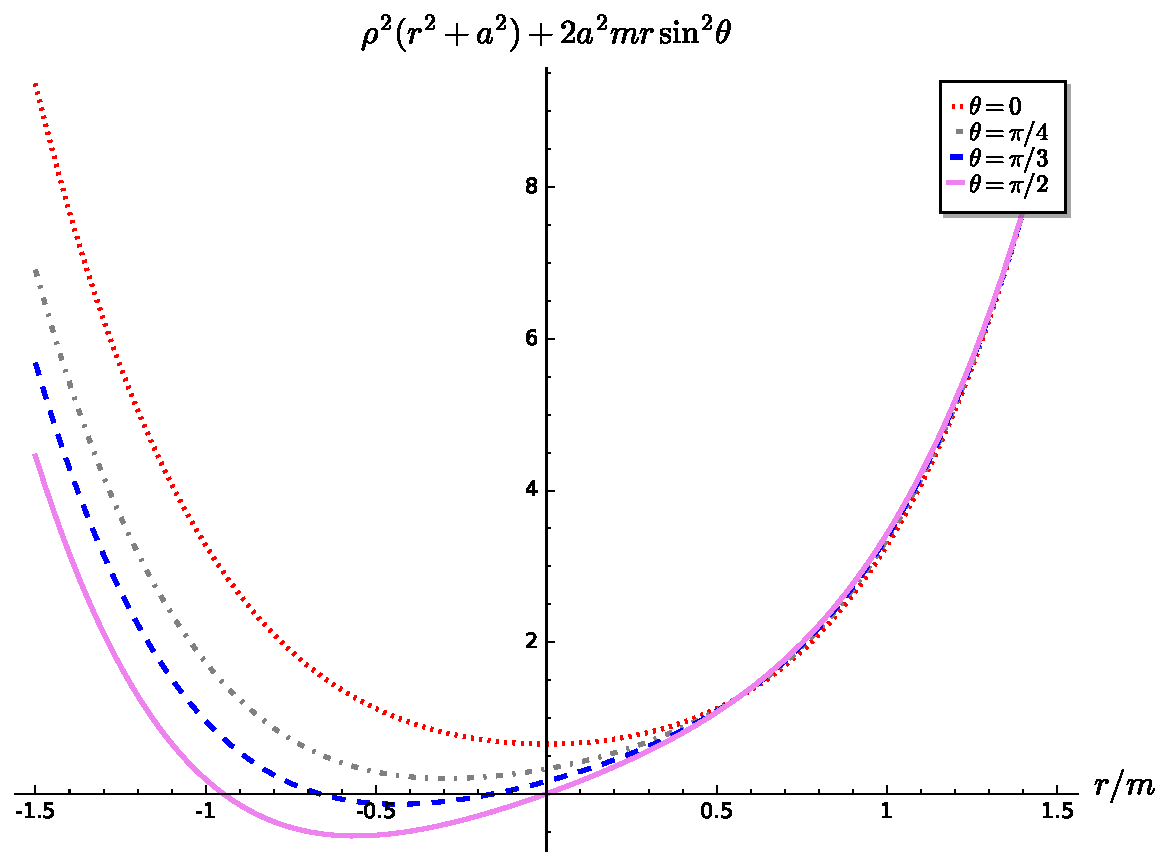
\includegraphics[width=0.7\textwidth]{ker_sign_gpp.pdf}}
\caption[]{\label{f:ker:sign_gpp} \footnotesize
Graph of the function giving the sign of $g_{\ph\ph}$ for $a=0.9m$
and various values of $\theta$.}
\end{figure}

\subsection{Carter time machine}

Let us now focus on the second Killing vector, $\w{\eta}$.
From (\ref{e:ker:metric_BL}) and (\ref{e:ker:def_rho2}), we have
\[
    \w{\eta}\cdot\w{\eta} = g_{\ph\ph} = \left( r^2 + a^2 + \frac{2 a^2 m r \sin^2\th}{r^2 + a^2\cos^2\th} \right) \sin^2\th .
\]
Hence
\[
    \w{\eta}\ \mbox{spacelike} \iff
        (r^2 + a^2)(r^2 + a^2\cos^2\th) + 2 a^2 m r \sin^2\th > 0 .
\]
For $\theta\rightarrow 0$ or $\theta\rightarrow\pi$, the left-hand side of the above equality
is always positive, but for $\theta=\pi/2$ and $r$ negative with $|r|$
small enough so that $2 a^2 m |r| > r^2(r^2 + a^2)$, it is negative. This feature
is apparent on Fig.~\ref{f:ker:sign_gpp}: for $\theta$ close to $\pi/2$,
there is a region $\mathscr{T}$ defined by $r_{\mathscr{T}}(\theta) < r < 0$ for some
negative function $r_{\mathscr{T}}(\theta)$, such that $g_{\ph\ph}<0$.
Since $\mathscr{T}$ corresponds to negative values of $r$, we have
$\mathscr{T}\subset \M_{\rm III}$.
Hence we conclude:
\begin{itemize}
\item $\w{\eta}$ is spacelike in all $\M_{\rm I}$ and $\M_{\rm II}$, as well
as outside the region $\mathscr{T}$ in $\M_{\rm III}$;
\item $\w{\eta}$ is timelike in the subset $\mathscr{T}$ of $\M_{\rm III}$;
\item $\w{\eta}$ is null at the boundary of $\mathscr{T}$.
\end{itemize}
The region $\mathscr{T}$ is called
\defin{Carter time machine}\index{Carter!time machine}\index{time!machine (Carter)}.
This name stems from the fact that, thanks to $\mathscr{T}$, there is
a future-directed timelike curve connecting any two points of $\M_{\rm III}$
(see e.g. Proposition~2.4.7 of O'Neill's textbook \cite{ONeil95} for a
demonstration, or Carter's original article \cite{Carte68}).

\subsection{Singularities}

The components $g_{\alpha\beta}$ of the Kerr metric as given by  (\ref{e:ker:metric_BL})
are diverging at various locations:
\begin{itemize}
\item when $\rho^2\rightarrow 0$, which, given (\ref{e:ker:def_rho2})
and assuming $a\not=0$, is equivalent to approaching
the cylinder $\ring$ defined by (\ref{e:ker:def_ring});
\item when $\Delta\rightarrow 0$, which, given (\ref{e:ker:def_Delta}), is equivalent to either $r\rightarrow r_-$
or $r\rightarrow r_+$; the first case corresponds to the boundary (within $\R^2\times\SS^2$)
between $\M_{\rm II}$ and $\M_{\rm III}$ and the second case to the boundary
between $\M_{\rm I}$ and $\M_{\rm II}$.
\end{itemize}
The Kretschmann scalar is
\be
    K = 48 m^2\, \frac{r^6 - 15 r^4 a^2\cos^2\th + 15 r^2 a^4 \cos^4\th - a^6\cos^6\th}{(r^2+a^2\cos^2\th)^6}
\ee
